\section{Problem III}

\textbf{Solution:} \\\\
Since finding the $k$th largest element in the union of the two arrays is equivalent of finding the $n - k + 1$th smallest element. To easier analyze the algorithm we are going to apply, we denote $k^* = n - k + 1$.\\

Binary search is a good example of achieving logarithmic complexity by halving its search space in each iteration. As a good hint, to achieve complexity of $O(logn)$ running time, we must halved the search space of A and B in each iteration.\\

Base case is pretty strait forward: If length of one of the array is 0, then the answer is $k*$th smallest element of the second array.\\

Array $A$ and array $B$ could be described as follows:

\begin{figure}[h]
\centering
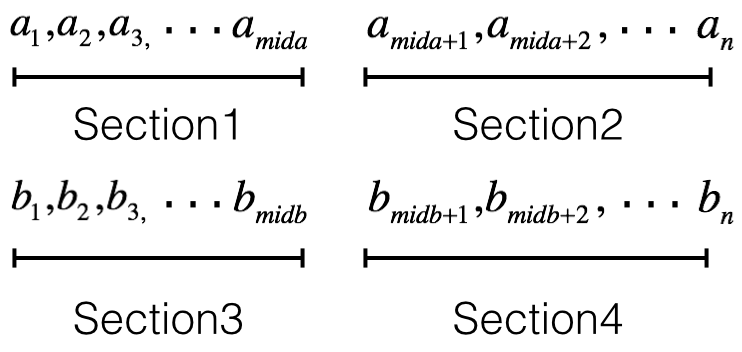
\includegraphics[scale=0.4]{hw2p3}
\caption{Picture of putting balls into bins}
\label{fig:p3}
\end{figure}

where $mida$ is the mid index of the first array $A$ and $midb$ is the mid index of the second array $B$. \\

If $mida + midb < k^{*}$, then it means that the $k^*$ smallest element is at \{Section1, Section2, Section4\} or \{Section2, Section3, Section4\}, the reason is as follows. If $A[mida] > B[midb]$, we can safely discard section3 since every element of section3 is smaller than $A[mida]$ and cannot be the $k^{*}$th smallest element of the union array. Similarly, If $A[mida] < B[midb]$ then we can discard section1.\\

However, if $mida + midb > k^{*}$, then it means that the $k^*$ smallest element is at \{Section1, Section2, Section3\} or \{Section1, Section3, Section4\}, the reason is as follows. If $A[mida] < B[midb]$, we can safely discard section4 since every element of section4 is bigger than $A[mida]$ and cannot be the $k^{*}$th smallest element of the union array. Similarly, If $A[mida] > B[midb]$ then we can discard section2.\\

The pseudo code is as follows:\\
[10cm]

\begin{algorithm}
\caption{Find($A$, $B$, $k^{*}$), $k^{*} = n - k + 1$}\label{euclid}
\begin{algorithmic}
\If {\textit{length(A)} = 0} \Return $B[k^{*}]$
\EndIf
\If {\textit{length(B)} = 0} \Return $A[k^{*}]$
\EndIf
\State $mida \gets length(A)/2$
\State $midb \gets length(B)/2$
\If {$mida + midb < k^{*}$} 
	\If {$A[mida] > B[midb]$}  $Find(A, B[midb + 1:], k^{*} - midb - 1)$\\
	// \textit{B[midb + 1:] means subarray after index of midb}
	\Else  $Find(A[mida + 1:], B, k^{*} - mida - 1)$\\
	// \textit{A[mida + 1:] means subarray after index of mida}
	\EndIf
\Else 
	\If {$A[mida] > B[midb]$}  $Find(A[:mida], B, k^{*})$\\
	// \textit{A[:mida] means subarray before index of mida}
	\Else  $Find(A, B[:midb], k^{*})$\\
	// \textit{B[:midb] means subarray before index of midb}
	\EndIf
\EndIf
\end{algorithmic}
\end{algorithm}

Since we halved the search space of A and B in each iteration, in the worst case we may halved both $A$ and $B$ down to empty which will cost $log(n_1) + log(n_2) = 2logn$. so the time complexity is $O(logn)$